\documentclass{article}
\usepackage{preamble}
\setlength\parindent{15pt}
\usepackage[
backend=biber,
style=alphabetic,
sorting=ynt
]{biblatex} %Imports biblatex package
\addbibresource{sample.bib} %Import the bibliography file

\title{Unit 6: Constellations}
\author{Astronomy at Cypress Springs High School}
\date{Updated on \today}

\numberwithin{equation}{section}
\setcounter{section}{6}
\numberwithin{figure}{section}

\usepackage{fancyhdr}
\pagestyle{fancy}
\renewcommand{\headrulewidth}{0pt}
\renewcommand{\headruleskip}{0mm}
\fancyfoot[C]{Access for free at \href{https://openstax.org/books/astronomy-2e/pages/1-introduction}{https://openstax.org/books/astronomy-2e/pages/1-introduction}
\hfill \thepage}


\makenoidxglossaries

\newglossaryentry{constellation}{
    name=constellation,
    description={one of 88 sections that collectively cover the entire sky; a star patter that represents an object or character with its origins in ancient stories}
}

\begin{document}

\maketitle

\subsection{Introduction}

The backdrop for the motions of the ``wanderers'' in the sky is the canopy of stars. If there were no clouds in the sky and we were on a flat plain with nothing to obstruct our view, we could see about 3000 stars with the unaided eye. To find their way around such a multitude, the ancients found groupings of stars that made some familiar geometric pattern or (more rarely) resembled something they knew. Each civilization found its own patterns in the stars. The ancient Chinese, Egyptians, and Greeks, among others, found their own groupings---or \textbf{constellations}---of stars. These were helpful in navigating among the stars and in passing their star lore on to their children.

\vspace{1ex}

You may be familiar with some of the old star patterns we still use today, such as the Big Dipper, Little Dipper, and Orion the hunter, with his distinctive belt of three stars. However, many of the stars we see are not part of a distinctive star pattern at all, and a telescope reveals millions of stars too faint for the eye to see. Therefore, during the early decades of the 20th century, astronomers from many countries decided to establish a more formal system for organizing the sky.

\begin{figure}[h!]
    \centering
    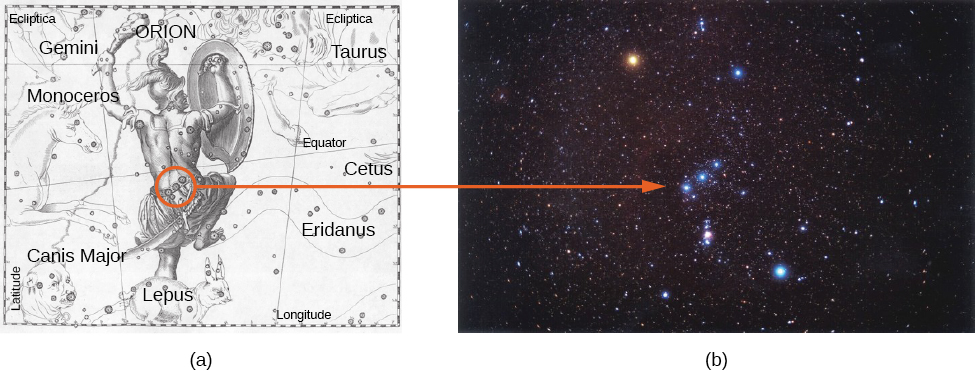
\includegraphics[width=0.8\textwidth]{Figures/Figure2.8.jpg}
\end{figure}

Today, we use the term constellation to mean one of 88 sectors into which we divide the sky, much as the United States is divided into 50 states. The modern boundaries between the constellations are imaginary lines in the sky running north-south and east-west, so that each point in the sky falls in a specific constellation. Like the states in the US, not all constellations are the same size. The modern constellation of \textbf{Orion} is a kind of box on the sky, which includes, among many other objects, the stars that made up the ancient picture of the hunter. Some people use the term asterism to denote an especially noticeable star pattern within a constellation (or sometimes spanning parts of several constellations). For example, the Big Dipper is an asterism within the constellation of Ursa Major, the Big Bear.

\vspace{1ex}

Students are sometimes puzzled because the constellations rarely resemble the people or animals for which they were named. In all likelihood, the Greeks themselves did not name groupings of stars because they looked like actual people or subjects (any more than the outline of Washington state resembles George Washington). Rather, they named sections of the sky in honor of the characters in their mythology and then fit the star configurations to the animals and people as best they could.

\subsection{Orion, The Hunter}
Orion, the hunter, was the son of Poseidon, the Greek god of the sea (whose Roman counterpart is Neptune). Orion served as a hunter under King Oinopion in the island of Khios. One day, Orion raped the King's daughter, Merope, who may have been engaged to Orion. Upon hearing of this tragic news, King Oinopion blinded Orion and banished him from his kingdom and the island. 

\begin{figure}[h!]
    \centering
    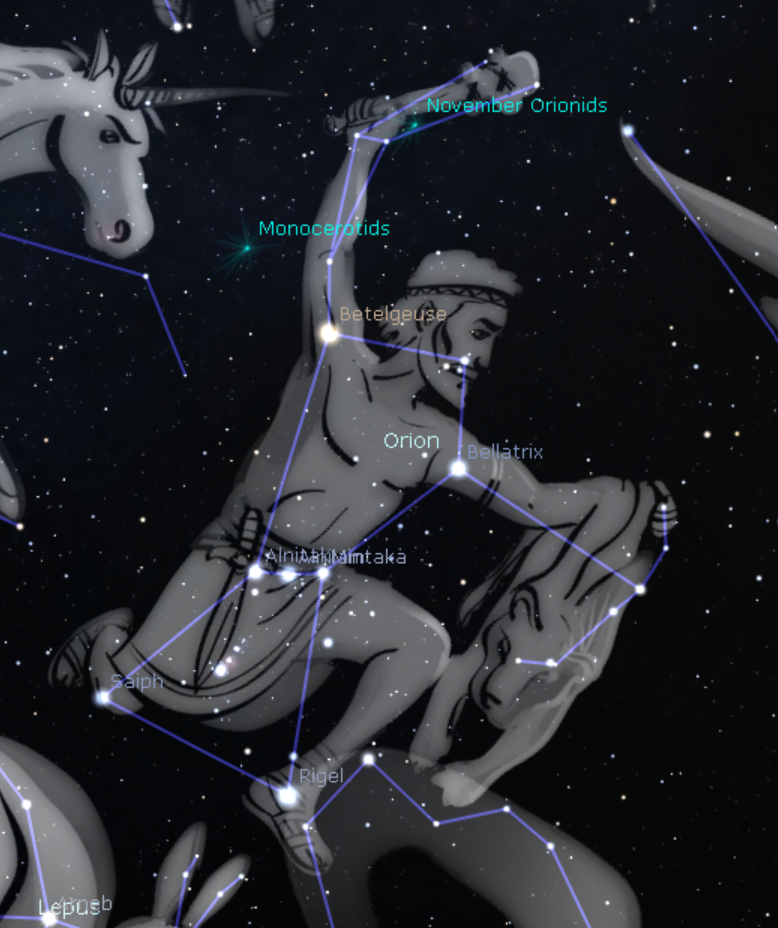
\includegraphics[height=7cm]{Figures/OrionArt.png}
\end{figure}

The now blinded Orion traveled across the sea to far away lands, in search of someone who could grant him back his vision. He was given a recommendation to travel eastward, to the place where the Sun rises. (How a blind person determines which way is east is not entirely clear. Perhaps he used his body to feel the heat from the Sun in the early hours of the morning.) Traveling east, Orion eventually encountered Helios, the Greek god of the Sun. (Hence, \textit{helio}centrism means Sun-centered.) Helios granted back Orion's vision, and Orion swiftly returned to Greece to take his revenge on King Oinopion for having blinded him. The King was no where to be found. Some say he hid underground in a bronze chamber. 

\vspace{1ex}

With no business left in Khios, Orion traveled to another Greek island, Delos (or possible Krete). Here he met another hunter whose hunting skills were on par with Orion's: the goddess Artemis. Orion and Artemis became hunting partners. After some time, Orion bragged to Artemis that he was determine to slay all animals and beasts in the world. Upon hearing of this, the great goddess Gaia, Mother Earth, sent Scorpius, the giant scorpion, to hunt down Orion. Together, Orion and Scorpius are immortalized in the celestial sphere as two constellations on opposite sides of the sky: when Orion sets in the west, Scorpius rises in the east, giving the impression that the scorpion eternally chases the hunter.


\begin{figure}[h!]
    \centering
    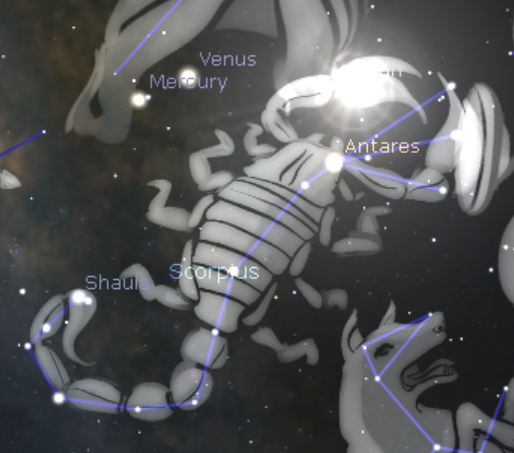
\includegraphics[width=7cm]{Figures/Scorpius.png}
\end{figure}

\subsection{Ursa Major \& Ursa Minor: Big Bear \& Little Bear}
In Greek mythology, Zeus is the god of the sky and thunder, and is sometimes considered the father of all other gods. Zeus was married to the goddess Hera, who was associated with many things including marriage, women, and childbirth. Incidentally, Hera was also Zeus's sister. While married to Hera, Zeus was seeing other goddesses and women. One of his mistresses was Callisto, a princess from the land of Arcadia, who (like Orion, the Hunter) was the hunting partner of the goddess Artemis. Zeus and Callisto were in love, and they bore a child named Arcus, who grew up to be a great hunter.

\vspace{1ex}

After learning about Zeus's infidelity and about the child that Zeus had with Callisto, Hera became enraged. In a fit of jealousy, Hera found Callisto and turned her into a bear. Arcus was destined to never see his mother again.

\vspace{1ex}

Years later, Arcus is now a young man and a highly skillful hunter, lethal with a bow and arrow. One day he is hunting in a forest when he comes across a giant bear. Being the keen hunter that he is, Arcus is determined to hunt down and kill the bear, all while being completely oblivious to that fact that the bear is Callisto, his mother. Callisto, the bear, having immediately recognized her son, begins trotting towards him to say hello. She stops in her tracks when she sees Arcus in the distance carefully pointing a bow and arrow in her direction. She turns around and trots away as fast as she can, as Arcus sprints closely behind her. 

\vspace{1ex}

Callisto manages to lead Arcus into the sacred temple of Zeus. Inside, Callisto the bear and her son Arcus cause a major disturbance to the otherwise peaceful temple. Zeus, upon hearing the great commotion, descends down to this temple to see what's going on. He notices his son Arcus and recognizes the bear as Callisto. Putting 2 and 2 together, he realizes that Arcus is unknowingly trying to kill his own mother. In order to prevent this tragedy, and in order to distance Callisto from the jealous wrath of Hera, Zeus turned his son Arcus into an little bear and placed both Arcus and Callisto in the sky, in the celestial sphere. Callisto and Arcus are Ursa Major and Ursa Minor, the big bear and little bear, two constellations that will always revolve closely around each other.

\begin{exercise} \label{9p6hLr}
    Look up the flag of Alaska. What does it look like? What is connection to the flag and the constellations of Ursa Major and Ursa Minor?
\end{exercise}

\begin{exercise}
    Using the \texttt{Stellarium} app, find Ursa Major and Ursa Minor. Draw a quick sketch of the stars and lines in these two constellations.
\end{exercise}

\clearpage
\subsection{Answers to Select Exercises}

\ref{9p6hLr}. The Alaskan flag contains the Big Dipper, which is a famous asterism in Ursa Major, two of whose stars point to Polaris, the North Star, which is the tip of the tail of Ursa Minor.


\end{document}